\documentclass[11.5pt]{article}
\usepackage[utf8]{inputenc}
\usepackage[T1]{fontenc}
\usepackage[textwidth = 460pt,top = 80pt, bottom = 80pt]{geometry}
\usepackage{graphicx}
\usepackage[justification=default]{subfig} %Manage sub-figures 
\usepackage[update]{epstopdf}
\usepackage[labelfont=bf]{caption}
\usepackage[dvipsnames]{xcolor}
\usepackage{fancyhdr}
\usepackage{booktabs}
\usepackage{multicol}
\usepackage{multirow}
\usepackage{titling}
\usepackage{bm}
\usepackage[leqno,fleqn,intlimits]{empheq}

%Bibliography

\usepackage{csquotes}
% \usepackage[sorting=none,%
% sortcites=true,%
% bibencoding=ascii,%
% autopunct=true,%
% hyperref=true,%
% language=auto,%
% %backref=true,%
% url=false,%
% %maxcitenames=10,%
% %minbibnames = 20,%
% maxbibnames = 3,%
% giveninits, 
% natbib = false,
% isbn=false,%
% backend=biber]{biblatex}
% \addbibresource{bibliography.bib}

\usepackage[]{hyperref}
\usepackage{cleveref}
%%% CREF setup
\crefname{equation}{Eq.}{Eqs.}
\crefname{table}{Table}{Tables}
\crefname{figure}{Fig.}{Figs.}


\begin{document}

\begin{titlingpage}
    \begin{center}
        \begin{figure}
            \centering
            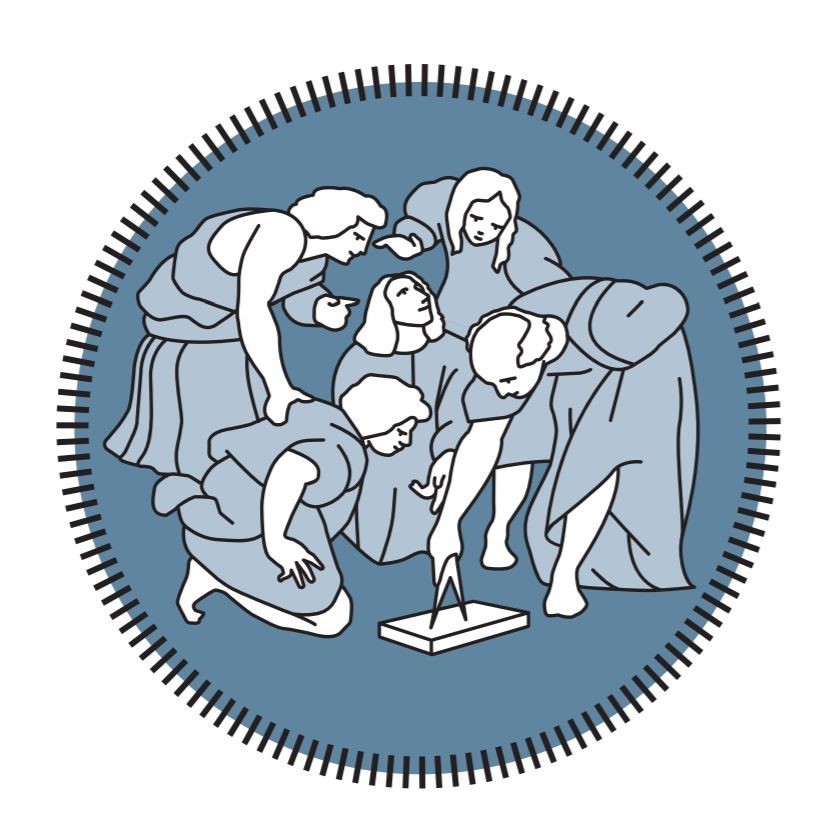
\includegraphics[width=0.6\textwidth]{graphics/logopolimi_mod.jpg}
        \end{figure}
        \Large{\textsc{Politecnico di Milano \\ School of Industrial and Information Engineering \\ M.Sc. in High Performance Computing}}

        \vspace{1cm}

        \rule{0.95\textwidth}{0.7mm}
        {\Large{\textbf{Final project: \\Classify musical genre using audio files}}}
        \rule{0.95\textwidth}{0.7mm}

        \vspace{1cm}

        \large{Prof. Edie Miglio \\ A.Y. 2024-2025}
    \end{center}

\end{titlingpage}

\pagenumbering{roman}

\tableofcontents

\clearpage

\setcounter{page}{1}
\pagenumbering{arabic}

\section{Introduction} \label{sec:introduction}
This project is a C++ implementation of the Randomized Singular Value Decomposition (rSVD) algorithm. We only used the matrix operations of the Eigen library to implement our algorithm. We do some benchmarks to compare the performance of our implementation with the Eigen library, the result indicates that our implementation can enhance the performance of handling large or sparse matrices.


\clearpage

% \printbibliography[heading=bibintoc, title = {References}]
\end{document}